\documentclass{article}
\usepackage[utf8]{inputenc}
\usepackage{listings}
\usepackage{xcolor}
\usepackage{tikz}
\usetikzlibrary{positioning, shapes.multipart}

\begin{document}

\noindent
\begin{minipage}[t]{0.45\textwidth}
\begin{lstlisting}[language=C++, basicstyle=\ttfamily\footnotesize, frame=single]
__global__ void kernel() {
    if (threadIdx.x % 2 == 0) {   
        // A
    } else {
        // B
    }
}
\end{lstlisting}
\end{minipage}
\hfill
\begin{minipage}[t]{0.5\textwidth}
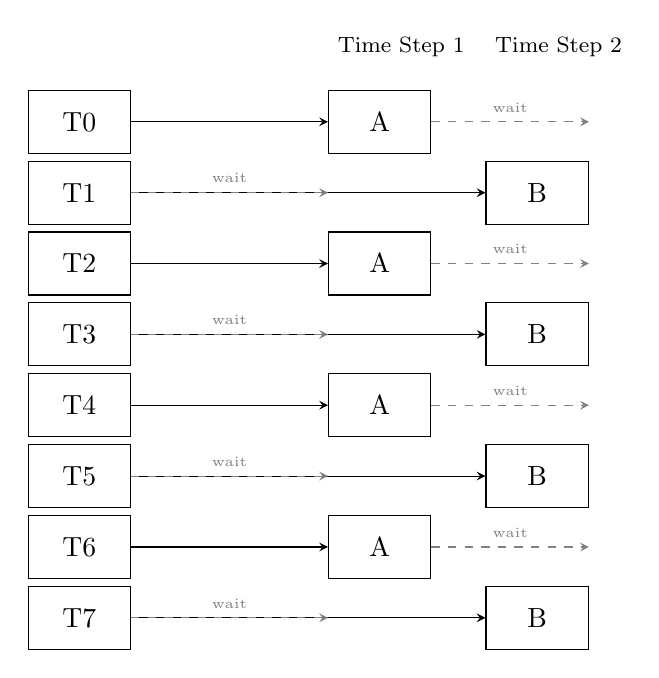
\begin{tikzpicture}[
    thread/.style={rectangle, draw, minimum width=1.3cm, minimum height=0.8cm, align=center},
    label/.style={font=\footnotesize},
    ->, >=stealth
]

% Threads
\foreach \i in {0,1,2,3,4,5,6,7} {
    \node[thread] (t\i) at (0, -0.9*\i) {T\i};
}

% Time labels
\node[label, above right=0.3cm and 2.5cm of t0] {Time Step 1};
\node[label, above right=0.3cm and 4.5cm of t0] {Time Step 2};

% A path (even threads)
\foreach \i in {0,2,4,6} {
    \node[thread, right=2.5cm of t\i] (a\i) {A};
    \draw[->] (t\i) -- (a\i);
}

% B path (odd threads)
\foreach \i in {1,3,5,7} {
    \node[thread, right=4.5cm of t\i] (b\i) {B};
    \draw[->] (t\i) -- (b\i);
}

% Dashed arrows to show waiting
\foreach \i in {1,3,5,7} {
    \draw[dashed, gray, ->] (t\i.east) -- ++(2.5,0) node[midway, above, sloped] {\tiny wait};
}

\foreach \i in {0,2,4,6} {
    \draw[dashed, gray, ->] (a\i.east) -- ++(2.0,0) node[midway, above, sloped] {\tiny wait};
}

\end{tikzpicture}
\end{minipage}

\end{document}

